\documentclass[11pt,a4paper]{article}
\usepackage[margin=25mm]{geometry}
\usepackage{fontspec}
\setmainfont{Latin Modern Roman}
\usepackage{microtype,booktabs,longtable,array,graphicx,xcolor,hyperref}
\definecolor{ceraink}{HTML}{13202B}
\definecolor{ceratealtext}{HTML}{0B6F6A}
\hypersetup{colorlinks=true,linkcolor=ceratealtext,urlcolor=ceratealtext,citecolor=ceratealtext}
\setlength{\parskip}{0.5em}
\setlength{\parindent}{0pt}
\emergencystretch=2em
\title{Counterexample-Guided Repair of Learned Rewards\\\large Project report for review}
\author{Varun Aditya \and Ravi R Naidu}
\date{18 November 2026}
\begin{document}
\begin{center}
\includegraphics[height=14mm]{figures/logo-mark.pdf}\end{center}
\maketitle
\begin{abstract}
A search guided by a learned model can select protein variants whose predicted fitness is high but whose measured fitness is less favorable. This project builds and evaluates a retrospective prototype that records warning signals and tests bounded changes to its selection rule. The system uses fixed protein-sequence representations, an ensemble of regressors, prediction ranges, predefined repair options and locally enforced checks. Experiments use existing public measurements rather than new laboratory measurements. In a four-protein comparison, each of two repair policies obtained a higher final best score than fixed reward in zero of 40 matched starts, tied in 35 and scored lower in five. Repair frequently stopped earlier, so these results combine the effects of the repair policy and different measurement counts. Additional shift-focused studies and prediction checks expose further weaknesses. The work establishes a reproducible research prototype and reports negative results; it does not demonstrate that repair improves protein engineering outcomes.
\end{abstract}
\setcounter{tocdepth}{1}
\begingroup\small\tableofcontents\endgroup
\newpage
\section{Problem and objective}
A protein variant is an amino-acid sequence changed from a reference sequence. Its fitness is an experimentally measured property such as activity or stability; the exact meaning and scale depend on the dataset. A laboratory measurement can be expensive, so a model may predict fitness and help choose which variants to measure next. The danger is that an optimizer can repeatedly choose variants where its model is inaccurate.

The project asks whether a search can record signs of model or reward failure, propose a limited change to its scoring rule, and retain the change only after defined checks. The synopsis proposed five warning categories, comparison with several search methods, and evaluation under different kinds of dataset shift. This report distinguishes implemented mechanisms from evidence of effectiveness. A warning is an operational signal; it is not automatically proof of a biological failure.

\section{Relation to existing research}
ProteinGym provides a broad benchmark for prediction and design and evaluates multiple aspects of ranking and discovery rather than relying on one score \cite{proteingym}. FLIP2 supplies protein datasets and deliberately different train/test splits, including mutation-count and fitness-defined splits \cite{flip2}. These benchmarks motivate reporting each protein and split separately. The WILDS benchmark illustrates why performance on a different population can differ from performance on training-like examples \cite{wilds}. It does not validate any CERA result.

Prediction ranges are constructed from errors on reserved measurements. Conformal prediction is useful for constructing such ranges, but its usual coverage statements depend on assumptions about the relationship between calibration and future examples \cite{conformal}. In this project, the search chooses future variants adaptively and the Hydro split is defined using fitness; observed coverage is therefore reported rather than promised. The study is a finite-pool simulation, so findings concern the available measured variants, not all possible protein sequences.

\section{Data and preparation}
\begin{center}
\begin{tabular}{@{}p{3.1cm}p{1.8cm}p{7.4cm}@{}}
\toprule
Dataset & Local rows & Use and limitation \\
\midrule
Alpha amylase & 3,706 & Development; previously measured activity. \\
Imine reductase (IRED) & 8,586 & Evaluation; the released split distinguishes variants by number of substitutions. \\
Hydrophobic core (Hydro) & 24,935 & Evaluation; three proteins are analyzed separately and the low-to-high split is based on measured fitness. \\
\bottomrule
\end{tabular}
\end{center}
The local IRED split matches the current official split download byte for byte. The benchmark website describes 17,143 variants, which is the laboratory's full screened set: 10,905 active variants plus 6,238 inactive ones reported in the original preprint. The local split contains only measured-active variants without flagged insertion, deletion or stop-codon rows, plus a limit on the number of changes; 865 of the preprint's inactive variants are missing from the laboratory's pinned inactive table and remain unexplained. Data sources, licenses, references and fingerprints are recorded in \href{../data/SOURCES.md}{data/SOURCES.md} and \href{../docs/data/ired_preparation.md}{the IRED preparation notes}.

The search limits eligible sequences to at most four substitutions from the relevant reference. A fixed ESM-2 model converts a sequence into 320 numbers, called a representation. Caches are checked against recorded data and model fingerprints. The measured scores are hidden from the supported search interface until selected, although the source files are accessible to a person with local file access. The implementation is not an adversarially secure data enclave.

\section{System design}
\begin{figure}[ht]
\centering
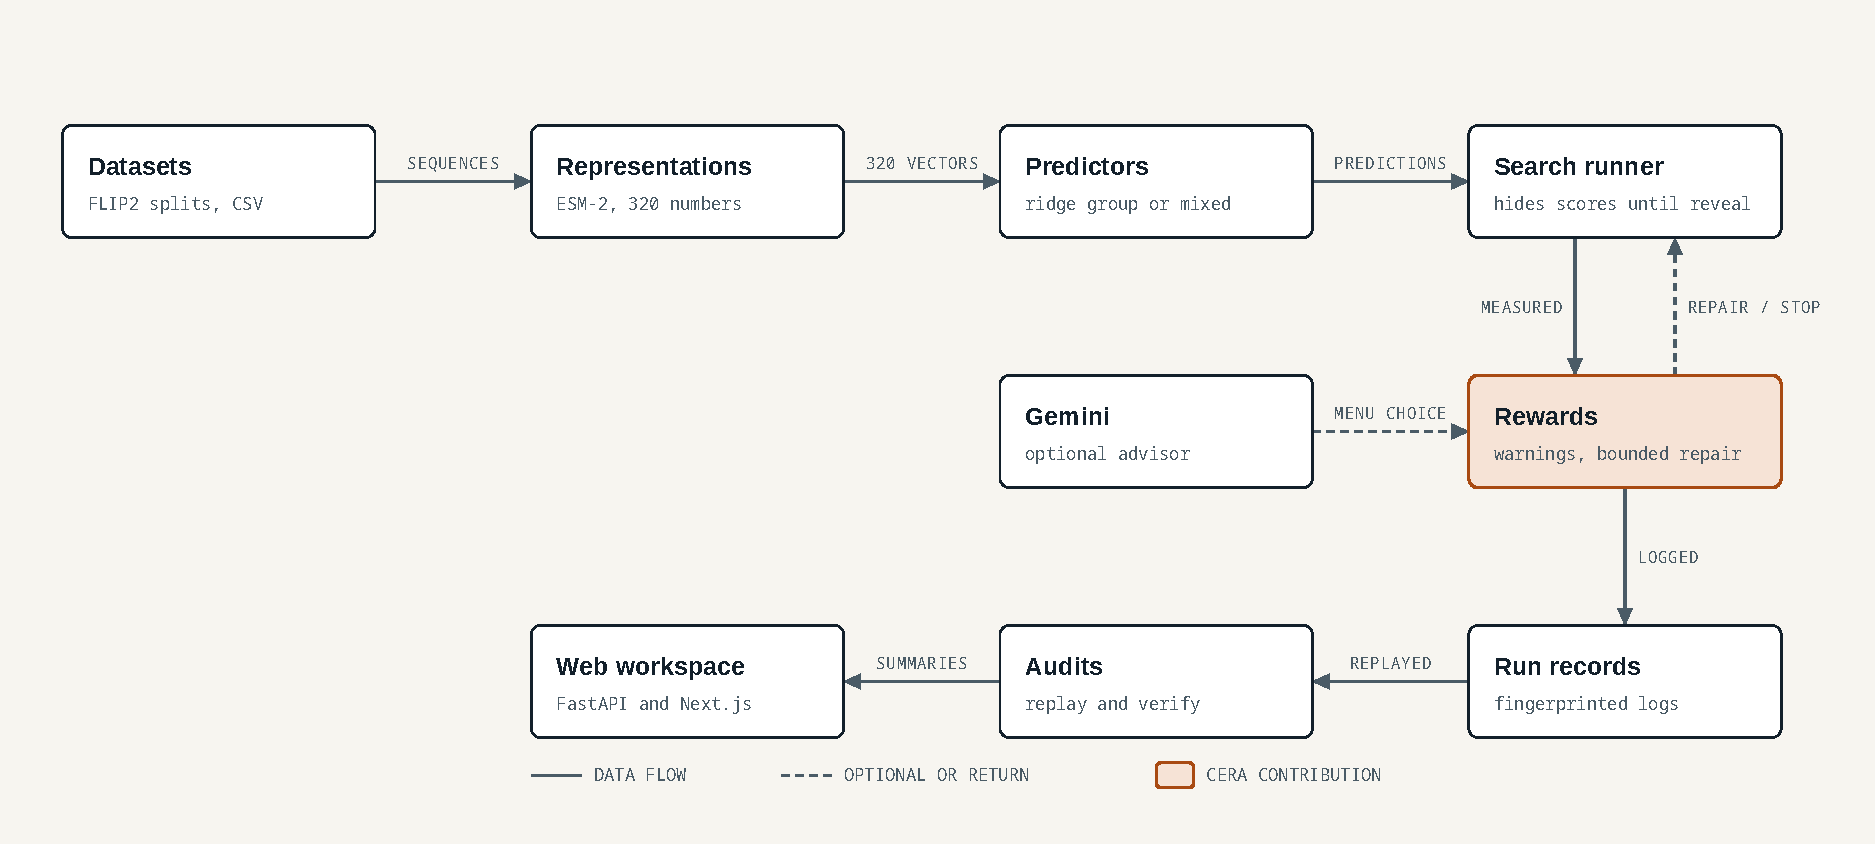
\includegraphics[width=\linewidth]{figures/architecture.pdf}
\caption{CERA architecture. Datasets feed representations and predictors, the search runner reveals scores, the rewards layer raises warnings and repairs, and run records are replayed by audits and shown in the web workspace.}
\end{figure}
\subsection{Prediction and selection}
The main experiments fit five ridge regressors to revealed measurements. Ridge regression limits the size of fitted weights; each member is fitted on a bootstrap sample. The mean prediction estimates fitness and variation between members is used as a model-disagreement signal. Twenty of the 100 starting measurements are reserved for setting prediction ranges; the remaining 80 are initially available for fitting. Models are refitted as new measurements are revealed.

The selection rule combines predicted fitness with an uncertainty penalty, a distance penalty and a batch-diversity bonus. Candidate sequences must satisfy the fixed mutation limit. A batch is selected without reading its unseen scores, and the recorded measurements are revealed afterward. The experimental mixed predictor replaces two ridge members with two small neural networks. The local workspace currently supports this mixed option for Amylase only.

\subsection{Warnings, repair and records}
The implementation records coverage, support, disagreement, constraint and diversity checks. For relevant warnings, it constructs a finite menu of allowed weight changes. A rule-based policy or Gemini can choose an ordering; local code checks each candidate change and can retain the old rule or stop after failed repairs. Gemini does not execute generated code. The reported repair cost is a dimensionless ordering score, not a currency amount.

The software records selections, pre-reveal predictions, observations, warnings, repair proposals and stop reasons. A separate decision check reconstructs selections and repair replays from recorded predictions. New local-web and matched-study Gemini repair records capture structured request details and returned text; older runs do not retain all raw responses, and complete prompt/response logging remains partial. Goal text entered by a user is sent to the configured provider and saved locally.

\section{Experimental design}
The main matched study used IRED and three Hydro proteins. For each of ten starting seeds per protein, nine methods received the same 100 initially revealed variants and a maximum of 100 additional measurements, in batches of ten. Starting sets were sampled from all eligible variants without using the benchmark split labels. The methods included random selection, greedy prediction, fixed reward, rule-based repair, Gemini-assisted repair, mean plus spread, expected improvement, finite-pool recombination and an AdaLead-style search. The latter acquisition and local-search baselines are adaptations to the available measured pool. All 360 runs reached a terminal runner status; a policy that stopped early is retained as an outcome, not counted as a failed execution.

Two later studies used different initial groups: IRED variants with at most two substitutions and Hydro variants from the lower-fitness side of its split. Later selections could come from all eligible variants. The Hydro start uses score-derived membership, information a real search would not normally have before measurement. IRED starting samples included validation-marked training-side rows. Neither study is an official static FLIP2 benchmark evaluation. Earlier test-side outcomes had already been inspected, making these analyses exploratory.

\section{Results}
\subsection{Four-protein comparison}
At each policy's actual stop, both repair policies had a higher best measured score than fixed reward in 0 of 40 paired starts, an equal score in 35 and a lower score in 5. A tie means an absolute score difference of at most $10^{-12}$. Fixed reward used all 100 new measurements in every run. Rule-based repair stopped after failed checks in 35 of 40 runs and Gemini-assisted repair in 36 of 40. The two repair policies matched in final best score across all pairs, which does not establish equivalence.

A later comparison read each fixed-reward run at the same number of new measurements as its paired repair run's stopping point. Each repair policy tied in 39 of 40 starts and had one lower score, on IRED. Four of the five actual-stop losses became ties at equal measurement counts. The analysis uses stopping points chosen by the repair policy and gives a descriptive comparison. See the \href{../docs/studies/multiprotein/four_protein_findings.md}{primary study findings} for the method and paired data.

The starting set already contained a top-one-percent eligible variant in 9 of 10 IRED starts, 8 of 10 P06241 starts, 7 of 10 P01053 starts and 9 of 10 P0A9X9 starts. This limits how well a simple yes/no top-one-percent hit can distinguish methods. The later recall analysis measures the fraction of the eligible top group found and includes initial observations; it is documented separately \cite{metrics}.

\subsection{Shift-focused searches}
In the IRED low-change-start study, each repair policy was higher than fixed reward in one pair, tied in seven and lower in two. Both repair policies stopped after failed checks in all ten runs and used 410 new measurements across the ten runs, compared with 1,000 for fixed reward.

In the Hydro low-fitness-start study, each repair policy tied fixed reward in five of 30 starts and scored lower in 25 at its actual stop. Each stopped after failed checks in 27 of 30 runs and used 1,130 new measurements versus 3,000 for fixed reward. A post-result comparison at the same measurement count found 30 tied best scores per policy. Neither comparison isolates a causal repair effect.

\subsection{Held-out prediction and the mixed predictor}
On the Amylase close-to-far position split, the five-ridge predictor had 90.2\% median coverage and median rank correlation of 0.0005 across ten starts on 1,709 eligible far-side variants. The \href{../docs/studies/amylase/position_shift.md}{position-shift check} assesses static prediction on development data.

A static check using ten starts per protein measured median prediction-range coverage of 90.0\% for IRED and 0.0\%, 11.7\% and 10.6\% for Hydro P06241, P01053 and P0A9X9, respectively. These are medians across starts on the same measured datasets, not independent biological replications or formal coverage guarantees.

The exploratory mixed-predictor comparison reused the same starting examples. Neither predictor showed a consistent advantage across the four groups. Both had low coverage on held-out Hydro variants \cite{mixed}.

\newpage
\subsection{Warning checks on known cases}
Precision is the fraction of warnings that matched a labeled positive case. Recall is the fraction of labeled positive cases that triggered a warning.

\begin{center}
\begin{tabular}{@{}p{3.6cm}p{5.7cm}rr@{}}
\toprule
Warning & Positive case & Precision & Recall \\
\midrule
Coverage & Moderate undercoverage & 239/245 & 239/1,000 \\
Coverage & Severe undercoverage & 946/952 & 946/1,000 \\
Unfamiliar candidates & Distant candidates, 10\% miss probability & 74/74 & 74/1,000 \\
Unfamiliar candidates & Distant candidates, 50\% miss probability & 943/943 & 943/1,000 \\
Model disagreement & One model swaps two ranks & Undefined & 0/45 \\
Model disagreement & One model reverses its ranking & 45/45 & 45/45 \\
Constraint & Hand-picked rule violation & 7/7 & 7/7 \\
Diversity & Hand-picked batch below the rule threshold & 2/2 & 2/2 \\
\bottomrule
\end{tabular}
\end{center}
The first six comparisons use equal numbers of constructed positive and reference cases. The unfamiliar-candidate reference cannot trigger by construction. Precision is undefined for the rank swap because no warning fired. The constraint and diversity cases test implementation. One single-variant diversity case was excluded because it had no pair to compare. These results apply to the tested cases. Accuracy on new laboratory outcomes remains unknown. The \href{../docs/overview/submission_readiness.md}{submission notes} link to the recorded counts.

\section{Interpretation and limitations}
Repair often stopped earlier than fixed reward, leaving less opportunity to discover higher-scoring variants. The local checks verify proposed changes against recorded evidence. The effect on future measurement coverage remains unestablished.

The data comprise prior experimental measurements. Independent laboratory validation of the warnings and repair benefit remains unavailable. Repeated starts reuse the same proteins. The four-substitution cap excludes some source variants. Hydro's score-defined starting split and IRED's included validation-marked rows limit comparison with an official benchmark. The additional mixed-model and post-result analyses are exploratory.

\paragraph{Recovery targets.} After the first accepted repair, 11 of 38 complete windows of 30 measurements met the 85--95\% coverage band. In a separate retrospective check, simple regret was the gap between the best score found and the best score in the eligible measured pool. Only six of 160 repair-policy runs had 30 later measurements after a coverage warning. Those six represent three matched starts under two policies. Each tied fixed reward at the same measurement count, yielding a 0\% reduction against the 10\% target. This subset leaves the original shift-split target unverified. The \href{../docs/overview/submission_readiness.md}{submission notes} provide denominators and paired records.

The prototype runs locally for a single user. Provider token counts are available for some calls. Earlier runs retained only the parsed responses and usage reported in their records.

\section{Implementation and reproducibility}
The backend is a Python package grouped by datasets, representations, predictors, experiments, rewards, provider integration, analysis, workspace services and provenance. Study scripts are modules of a \texttt{scripts} package, organised by topic (data, Amylase, repair, warnings, multi-protein, mixed predictor, held-out prediction and reporting), and tests are grouped by the same areas. The frontend exposes the dataset catalog, the recorded results, a local experiment workflow, run review and Amylase prediction. The project documentation is consolidated under \texttt{docs/} with a glossary; the \href{../docs/history/work_log.md}{work log} records decisions and checks, while the \href{../docs/overview/completion_review.md}{completion evidence review} maps the synopsis to the available evidence.

Saved run records store fingerprints of the data, caches and code that produced them. The repository was reorganised after the studies ran, so the original layout is kept under the git tag \texttt{pre-restructure}; \href{../docs/overview/reproducing_results.md}{reproducing results} explains how to verify older records. An audit of one saved Amylase repair comparison gave the same result (10 runs, 72 selections, 30 repair replays) from the original and the reorganised layouts.

After the reorganisation, all 189 earlier backend tests passed, and four new tests for the IRED selection check and the audit helpers bring the total to 193. The production frontend build and type check passed. After the visual redesign, an automated design sweep and an axe-core accessibility scan reported no violations on all eight routes at desktop and phone width, and a keyboard-only Chromium walkthrough submitted a real local experiment and read its result. The Tab order and focus indicators were checked; the accessibility tree was read for labels, groups and headings. No real screen reader (such as NVDA, Orca or VoiceOver) was run, so screen-reader behavior remains unchecked. The held-out mixed-model audit refitted 200 individual models on the same GPU and reproduced 67,660 predictions within an absolute tolerance of $10^{-5}$. This verifies reproducibility using the original implementation. A fresh audit checked all 360 primary-study records, reconstructing 2,943 batch selections and 549 repair replays. The regenerated evaluation report matched the committed report byte for byte.

\section{Conclusion}
CERA delivers a working retrospective research prototype with bounded reward changes, warning records and comparisons across multiple protein groups. The studies expose a meaningful failure mode: the tested repair policies frequently stopped early and did not improve final best scores over the fixed-reward baseline in the primary comparison. Static held-out checks also show poor prediction-range coverage in the shifted Hydro groups. These findings justify careful reporting of the implemented safeguards and their limits, not a claim of validated repair effectiveness. Further work would require independently justified failure labels, a design that separates repair from stopping, and new evaluation data before claiming generalization.

\begin{thebibliography}{9}
\bibitem{proteingym} P. Notin et al., ``ProteinGym: Large-Scale Benchmarks for Protein Fitness Prediction and Design,'' NeurIPS Datasets and Benchmarks, 2023. \url{https://papers.nips.cc/paper_files/paper/2023/hash/cac723e5ff29f65e3fcbb0739ae91bee-Abstract-Datasets_and_Benchmarks.html}
\bibitem{flip2} K. Didi et al., ``FLIP2: Expanding Protein Fitness Landscape Benchmarks,'' benchmark and datasets. \url{https://flip.protein.properties/}
\bibitem{wilds} P. W. Koh et al., ``WILDS: A Benchmark of in-the-Wild Distribution Shifts,'' ICML, 2021. \url{https://proceedings.mlr.press/v139/koh21a.html}
\bibitem{conformal} A. N. Angelopoulos and S. Bates, ``A Gentle Introduction to Conformal Prediction and Distribution-Free Uncertainty Quantification,'' 2021. \url{https://arxiv.org/abs/2107.07511}
\bibitem{metrics} CERA, ``Additional retrospective search metrics,'' project record. \href{../docs/studies/multiprotein/additional_metrics.md}{docs/studies/multiprotein/additional\_metrics.md}.
\bibitem{mixed} CERA, ``Mixed predictor: exploratory held-out protein comparison,'' project record. \href{../docs/studies/hybrid/mixed_heldout.md}{docs/studies/hybrid/mixed\_heldout.md}.
\end{thebibliography}
\end{document}
